\documentclass{article}
\usepackage{multirow}
\usepackage{Sweave}
\begin{document}
\Sconcordance{concordance:draft1.tex:draft1.Rnw:%
1 2 1 1 0 11 1 1 8 87 1 1 9 17 1 1 10 65 1 1 11 250 1}




\section*{Abstract}

Community-driven online question and answer forums (CQA) house an expansive amount of crowd-sourced knowledge in the form of thousands of questions and answers posted everyday. Forums can cover a broad range of topics, like \textit{Yahoo! Answers}, or can be focused on a specific topic, like computer programming-focused \textit{Stack Overflow}. An example of the latter is iFixit's \textit{Answers} forum. The \textit{Answers} forum features user-asked questions related specifically to device repair, which are answered by both repair experts and everyday users, furthering iFixit's mission to enable individuals to repair their own devices. As such, it is important that questions receive timely answers. This paper presents a survival analysis on the time until a question receives its first answer. We developed a Cox proportional hazards model to predict the failure probability of a question, or the probability that a question receives an answer before a certain time. Though we identified signifcant predictors, the predictive accuracy was low ($R^2 = 0.15$). Our findings indicate that the most important predictors were the device category of the question (questions pertaining to Apple products received answers faster than others (HR = 2.56, 95\% CI = (2.31, 2.82))) and factors related to the question's title (e.g., whether or not it was phrased as a question (HR = 1.31, 95\% CI = (1.22, 1.41))). Future studies could investigate if the factors identified as signifcant in our study can be generalized to other CQAs. 

%----------------------------------------------------------------------------------------------------

\section*{Introduction}

Community-driven online question and answer forums (CQA) are becoming widely used sources of information. These online platforms allow for anyone to ask or answer a question, regardless of their background or expertise level. Forums can receive around 40 million visits every month.
    
The CQA analyzed in this paper is iFixit's \textit{Answers} forum. Founded in 2003, iFixit's mission is to enable people to repair their broken devices, effectively saving them money and reducing electronic waste. The company provides over 30,000 free online repair guides and sells the specialized tools and parts needed for such repairs.
    
As not all possible repairs are covered in the published repair guides, and users may have questions related to those guides, iFixit's \textit{Answers} forum is another important resource. This platform features questions pertaining to over 9,000 devices with over 100,000 solutions. Questions range from broken devices like jammed zippers to shattered iPhone screens. As many rely on this forum for help with repairs, it is important that users receive timely answers. Fast response times will enhance user engagement and generate more web traffic, which is valuable to the reputation and longevity of the \textit{Answers} forum. Analysis of answer times can reveal factors that affect how quickly questions are answered, which can lead to suggestions for how users can ask better questions to minimize answer times, and for how the forum design can be improved. 
However, analysis and prediction of answer \textit{times} on CQAs have not been thoroughly investigated. As the majority of existing research focuses on assessing and predicting question and answer quality, there is need for further analysis of response times in these forums. This paper presents a survival analysis on the time until a question is answered on iFixit's \textit{Answers} forum, in order to determine factors significantly related to answer time and to predict the ``survival'' probability of a question.

%----------------------------------------------------------------------------------------------------

\section*{Related Work}
  
In regards to investigation of forum response times, \citep{Bhat2014} developed a classification model to analyze response times of questions posted on \textit{Stack Overflow}, and found that tag-based features like the number of tags included or the number of subscribers a certain tag has, were the best predictors of answer time. 

\citep{Mamykina2011} found that the swift answer times of \textit{Stack Overflow's} community is a result of the reputation system and the strict emphasis on factual and informative questions and answers, rather than discussion-based. 

\citep{Asaduzzaman2013} analyzed unanswered questions on \textit{Stack Overflow} to determine common characteristics and found that questions that went unanswered shared certain characteristics in that they were too short and vague, or utilized the tagging system incorrectly. 

%----------------------------------------------------------------------------------------------------

\section*{Materials}

good question ex: id 408124, 406786 (answered)
bad question ex: id 410310, 405882 (unanswered) 

The data analyzed contained 8,025 questions posted from April 8, 2017 (10:14 PM) to July 7, 2017 (9:28 PM) (the date the data was downloaded). Variables in the data included: device name and category, title, text, tags, whether or not the user was a member of iFixit's site for less than one day before the question was posted, date the question was posted, date the first answer was received. Variables derived: 

Categorical Variables: 

\begin{itemize}
  \item Device category the question pertains to. Categories include: Apple Products, Android\/Other Phone, PC, Tablet, Electronics, Camera, Vehicle, Game Console, Home, Other.
  \item Whether or not the question's title contains at least one word that is considered ``frequently used'' among answered questions. See appendix for a complete list of these terms. 
  \item Whether or not the question's title contains at least one word that is considered ``frequently used'' among unanswered question. See appendix for a complete list of these terms. 
  \item Whether or not the question's title ends in a question mark.
  \item Whether or not the question's text contains any end punctuation marks (. ? !). 
  \item Whether or not the question's text is in all lower case. 
  \item Whether or not the user edited or added information to the question's text sometime after posting it.
  \item Whether or not the user made an effort to solve the problem on their own, prior to asking the question.
  \item Day of the week the question was posted. 
\end{itemize}

Numeric Variables:

\begin{itemize}
  \item Average tag ``score'' for all of a question's tags. A tag score is defined as the proportion of times a tag appears in all of the data. Questions without tags were assigned a score of 0. 
  \item Average number of characters in each question's tags. 
  \item Number of characters in the question's text. 
  \item Number of characters in the user-defined device name. 
  \item Ratio of the number of line breaks to the number of characters in the question's text.
\end{itemize}

%----------------------------------------------------------------------------------------------------

\section*{Methods}

Questions analyzed were restricted to those posted in English. Time until event was defined as the time since posting until a question received its first answer. For questions that did not receive an answer by the download date, time until event values were defined as the time since posting to the time the data was downloaded. Such questions were considered right-censored, meaning that exact answer times for these questions are greater than the times in the data (questions can still receive answers after the download date) \citep{Kleinbaum2011}. 

Survival was defined as the event that a question did not receive an answer beyond a certain time, t. Estimates of survival probability were generated with the Kaplan-Meier method, which adjusts to the presence of right-censored, or unanswered questions \citep{Bland1998}. From these estimates, survival curves were constructed to examine the survival experience of questions. Mean, median and other percentiles of survival times were also generated. 

As the probability distribution for answer times was unknown, a nonparametric Cox proportional hazards model was developed to predict survival probability (Cox models are not based on an assumption of the shape of the underlying probability distribution) \citep{Moore2010}. To build the model, five-fold cross-validation was used. The full data was split into five training sets and five test sets \citep{sensitivity}. On one training set, distributions of all continuous variables were assessed and square root or log transformations were applied as necessary. Univariate analysis, performed on one training set, was used to identify variables to potentially include in the final Cox model \citep{Hammer}. Each categorical and continuous predictor was entered into separate univariate Cox models, and strength of association with answer times was assessed. Those with partial likelihood ratio test p-values of less than 0.001 were included in the final model. To investigate the use of splines on continuous predictors, univariate analysis was again performed. Continuous variables were fit to four separate univariate Cox models with: restricted cubic splines of three, four, and five knots, and no splines. AIC statistics were used to determine whether or not splines were necessary, as well as the optimum number of knots \citep{Harrell2015}. All predictors found to be significant in both stages of univariate analysis were included in the model for cross-validation. No variable selection was used, as \cite{Harrell2015} determined that reducing the number of predictors in the model harmed predictive accuracy, more so than leaving all predictors in. 

In each fold of cross-validation, the full model was built on the training set and used to generate predicted hazard ratios on the corresponding test set. To assess prediction performance, the predicted hazard ratios were entered into separate Cox models as the single quantitative predictor, with answer times as the survival time. The resulting estimated hazard ratio, R-square statistic, partial likelihood ratio and p-value were assessed as indicators of the model's performance. Signficant results would indicate high predictive accuracy. Concordance statistics and Somers' Dxy were also assessed to measure the model's discriminative ability \citep{Chen}. Concordance is defined as the probability that for any two randomly chosen questions, the question with the shorter survival time also has the higher predicted hazard. Concordance statistics close to 1 indicate high discriminative ability, while statistics close to 0.5 indicate discordance, or random predictions. Somers' Dxy is the difference between the model's concordance statistic and discordance, 0.5. A Somers' Dxy statistic of 0 indicates random predictions, while a statistic equal to 1 indicates perfect predictions \citep{Harrell2015}. These metrics were computed for each iteration on every training and test set. Averages of metrics across test sets were evaluated. The final model was then fit to the full data and the same metrics were computed and compared. 

Correlations between scaled Schoenfeld residuals, differences between observed and expected predictor values for questions that received answers, and a function of time, were examined to assess the proportional hazards assumption that the effect of predictors on hazard does not depend on time \citep{therneau}. Significant correlations would indicate that a predictor has violated this assumption . 

%----------------------------------------------------------------------------------------------------

\section*{Results}


% Distribution of answer times
\begin{figure}[h!]
  \includegraphics[scale=1]{times_dist.pdf}
  \caption{Distribution of answer times}
  \label{fig:answertimes}
\end{figure}

% Kaplan-Meier curve
\begin{figure}[h!]
  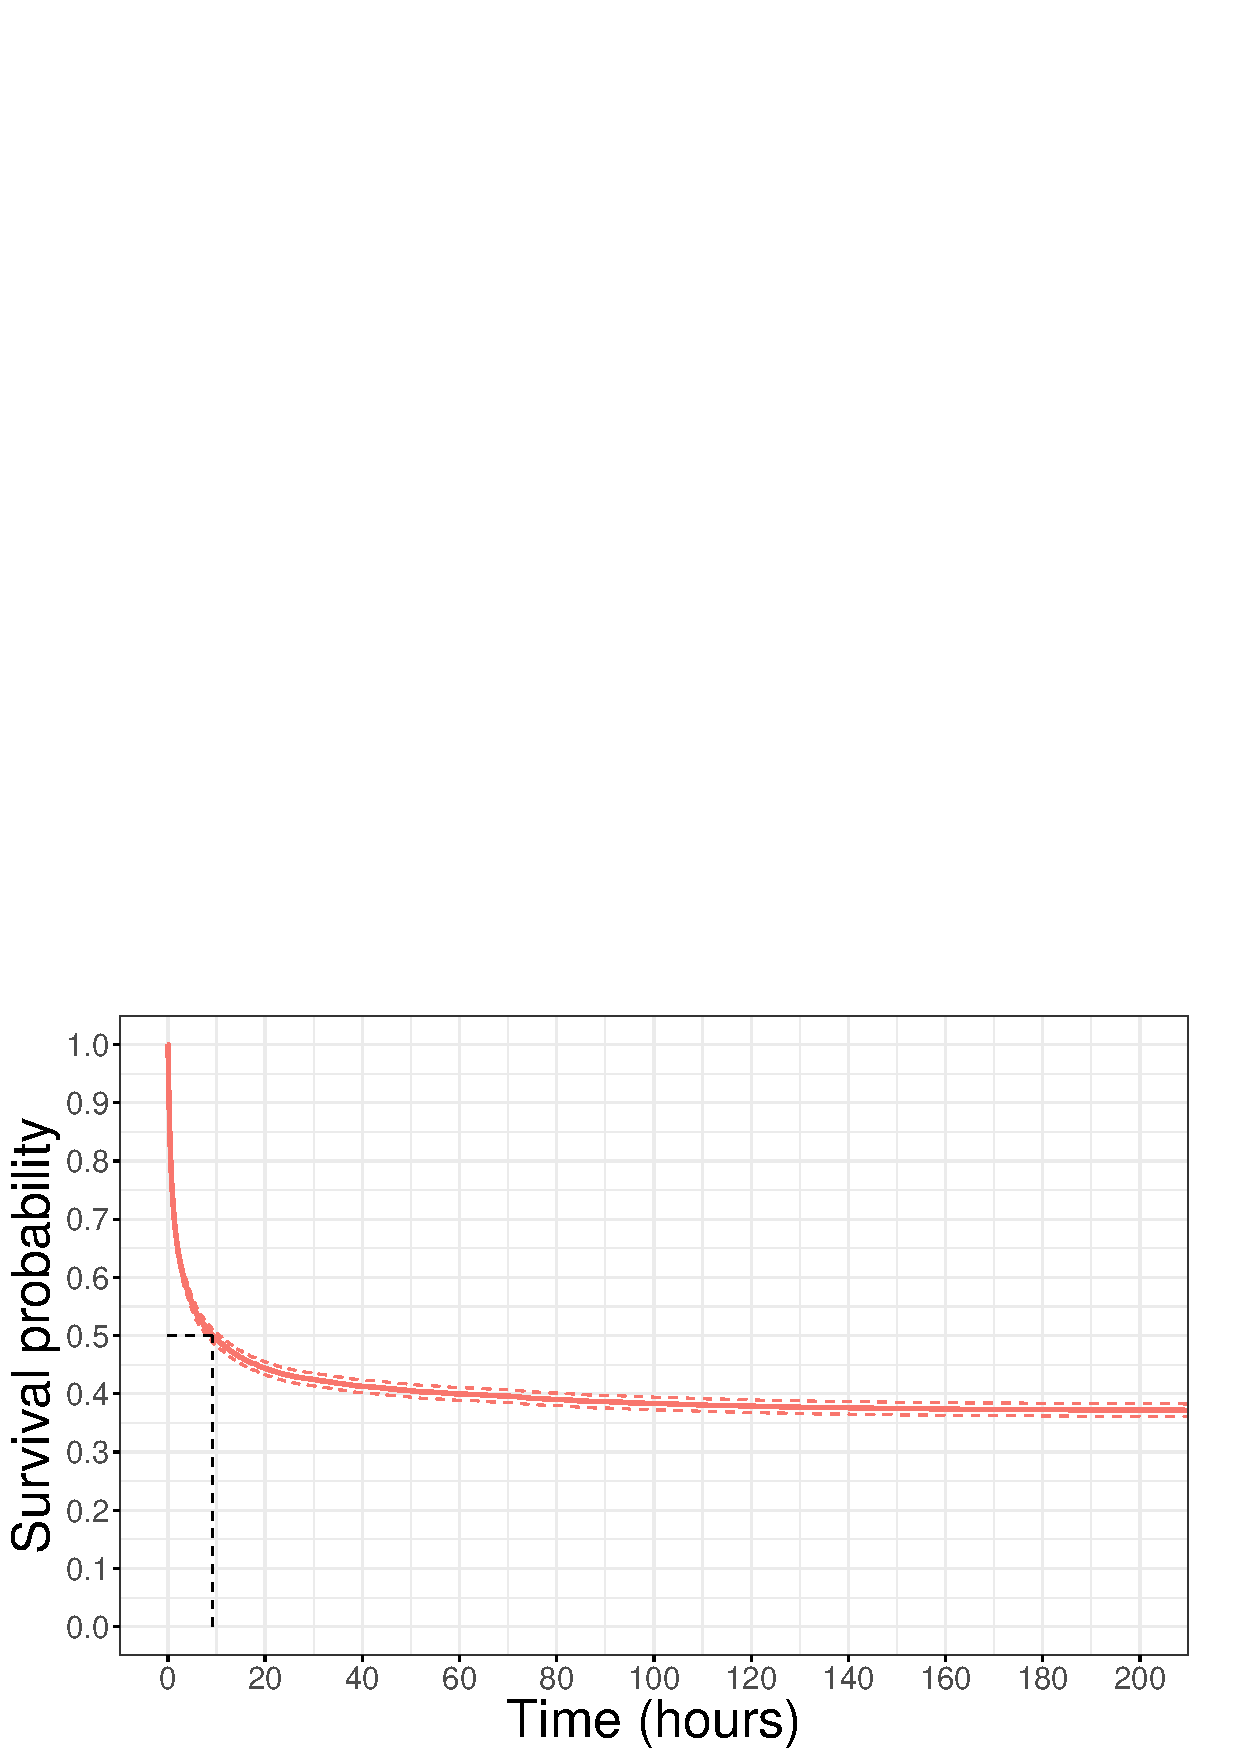
\includegraphics[scale=1]{kmcurve.pdf}
  \caption{Kaplan-Meier curve for all questions}
  \label{fig:kmcurve}
\end{figure}

  Of 8,025 questions in the full data set, 7760 were in English (97\% of the full data). Of those questions, 4951 (63.8}\%) received an answer by the download date. The shortest answer time was 0.5 hours. The longest was 2159.02 hours (89.96 days). Figure ~\ref{fig:answertimes} shows that the distribution of answer times for all questions is extremely right-skewed. 



% Table of percentiles 
\begin{table}[ht]
\centering
\begin{tabular}{rlr}
  \hline
 Percent\\ Answered & Time (hrs) \\ 
  \hline
  25 & 0.88 \\ 
  50 & 9.16 \\ 
  55 & 18.38 \\ 
  58 & 33.71 \\ 
  60 & 59.47 \\ 
  64 & 683.19 \\ 
   \hline
\end{tabular}
\caption{Table of Kaplan-Meier estimated quantiles of survival time}
\label{table:quantiles}
\end{table}

  Figure  ~\ref{fig:kmcurve} shows the Kaplan-Meier estimated survival probability for all questions in the data. The curve indicates that if a question does not receive an answer within the first 100 hours after it has been posted, the likelihood of it receiving an answer in the future is low. The Kaplan-Meier estimated mean survival time, or the average time until a question received its first answer was 775.75 hours, or 32.32 days. The median survival time, the time at which 50\% of the questions in the data received an answer, was 9.16 hours. Table \ref{table:quantiles} provides additional percentiles of survival time.

% Univariate analysis on quantitative predictors
\begin{table}[ht]
\centering
\caption{Univariate analysis results for quantitative predictors, ordered by increasing p-values} 
\begin{tabular}{|p{12cm}|p{2cm}|}
  \hline
  Predictor & p-value \\ 
  \hline \hline
  *Log transformation of the number of characters in a question's text & 0.00 \\ 
  \hline
  *Square root transformation of the number of characters in a question's text & 1.1102e-16 \\ 
  \hline
  Number of characters in a question's text (untransformed) & 6.9472e-12 \\
  \hline
  *Square root transformation of the ratio of the number of line breaks to the number of characters in a question's text & 1.1488e-11 \\ 
  \hline
  *Square root transformation of the average frequency ``score'' of a question's tags & 1.4642e-11 \\ 
  \hline
  Average frequency ``score'' of a question's tags (untransformed) & 1.2706e-08 \\ 
  \hline
  Ratio of the number of line breaks to the number of characters in a question's text (untransformed) & 1.3988e-7 \\ 
  \hline
  *Square root transformation of the number of characters in the user-defined device title & 2.2914e-4 \\ 
  \hline
  *Square root transformation of the average number of characters in a question's tags & 2.9999e-4 \\ 
  \hline
  Number of characters in the user-defined device title (untransformed) & 6.5304e-3 \\ 
  \hline
  Average number of characters in a question's tags (untransformed) & 2.6115e-2 \\ 
   \hline
\end{tabular}
\label{table:qresults}
\end{table}

% Univariate analysis on categorical predictors
\begin{table}[ht]
\centering
\caption{Univariate analysis results for categorical predictors, ordered by increasing p-values} 
\begin{tabular}{|p{12cm}|p{2cm}|}
  \hline
 Predictor & p-value \\ 
  \hline \hline
  Device category & 0.00 \\
  \hline
  Whether or not the user had been a member for less than one day before the question was posted & 0.00 \\ 
  \hline
  Whether or not the question's title contains terms considered to be frequently used among unanswered questions & 0.00 \\ 
  \hline
  Whether or not the question's title ended in a questionmark & 1.1423e-12 \\ 
  \hline
  Whether or not the question's text contained at least one end punctuation mark & 2.5354e-9 \\ 
  \hline
  Whether or not the question's text is in all lower case & 1.5400e-7 \\ 
  \hline
  Whether or not the user edited or added information to the question's text sometime after posting it & 2.5472e-7 \\ 
  \hline
  Whether or not the user made an effort to solve the problem on their own, prior to asking the question & 3.1648e-5 \\
  \hline
  Whether or not the question's title contains terms considered to be frequently used among answered questions & 7.6397e-5 \\ 
  \hline
  Day of the week the question was posted & 7.8677e-4 \\ 
   \hline
\end{tabular}
\label{table:cresults}
\end{table}


Each training set contained 6208 questions, and each test set contained 1552 questions. Results of univariate analyis, performed on one training set, for transformed and untransformed quantitative predictors, and categorical predictors, are are shown in Table \ref{table:qresults} and Table \ref{table:cresults}, respectively. All categorical predictors, as well as all continuous predictors marked with * were entered into the full model.

% Splines
\begin{table}[ht]
\centering
\caption{Determining the optimal k number of splines for each predictor} 
\begin{tabular}{| p{5cm} | l | l |}
  \hline
  Predictor & K & AIC \\ 
  \hline
  \multirow{ 4 }{ 5cm }{Log transformation of the number of characters in a question's text} 
  & 0 & 65862.83 \\ 
  & 5* & 65862.02 \\ 
  & 4 & 65863.35 \\ 
  & 3 & 65862.08 \\ 
  \hline
  \multirow{ 4 }{ 5 cm }{Square root transformation of the ratio of the number of line breaks to the number of characters in a question's text}
  & 0 & 65890.28 \\ 
  & 5 & 65884.70 \\ 
  & 4 & 65882.98 \\ 
  & 3* & 65881.93 \\ 
  \hline
  \multirow{ 4 }{ 5 cm }{Square root transformation of the average frequency ``score'' of a question's tags}
  & 0* & 65890.75 \\ 
  & 5 & 65891.69 \\ 
  & 4 & 65891.75 \\ 
  & 3 & 65892.35 \\ 
  \hline
  \multirow{ 4 }{ 5 cm }{Square root transformation of the number of characters in the user-defined device title}
  & 0 & 65922.76 \\ 
  & 5* & 65853.56 \\ 
  & 4 & 65882.07 \\ 
  & 3 & 65881.39 \\ 
  \hline
  \multirow{ 4 }{ 5 cm }{Square root transformation of the average number of characters in a question's tags}
  & 0 & 65923.26 \\ 
  & 5 & 65912.11 \\ 
  & 4* & 65910.10 \\ 
  & 3 & 65912.38 \\ 
   \hline
\end{tabular}
\label{table:splines}
\end{table}

Table \ref{table:splines} shows the results of determining the optimal number of knots for each quantitative predictor. Knots marked * were included in the final model. 

% Cross-validation metrics
\begin{table}[ht]
\centering
\caption{Average performance metrics for training and test sets} 
\begin{tabular}{rrrrrrrr}
  \hline
 & HR & LR & pval & R2 & AIC & Dxy & Concordance \\ 
  \hline
  Training Sets & 2.0164 & 937.2018 & 0.0000 & 0.1401 & 64752.0898 & 0.2693 & 0.6346 \\ 
  Test Sets & 1.9761 & 220.0417 & 0.0000 & 0.1401 & 13458.5808 & 0.2584 & 0.6292 \\
   \hline
\end{tabular}
\label{table:cv}
\end{table}

% Final metrics for full data 
\begin{table}[ht]
\centering
\caption{Performance metrics for model fit to the full data} 
\begin{tabular}{rrrrrrrr}
  \hline
  HR & LR & pval & R2 & AIC & Dxy & Concordance \\ 
  \hline
  2.0010 & 1192.3234 & 0.0000 & 0.1424 & 83128.2780 & 0.2698 & 0.6349 \\ 
   \hline
\end{tabular}
\label{table:finalmetrics}
\end{table}

Average performance metrics for test and training sets, found in Table \ref{table:cv}, were considerably low. However, metrics did not change substantially from training to test sets, indicating that the model does not overfit. The final model, with all variables described above including splines, was fit to the full data.

% Final model on full data
\begin{table}[ht]
\centering
\caption{Coefficients for predictors in the final model} 
\begin{tabular}{|p{1.5cm}|p{6cm}|p{2.5cm}|p{2.5cm}|}
  \hline
 Variable &  Levels & Hazard Ratios & p-value \\ 
  \hline
  \multirow{ 9 }{ 2 cm }{ Device Category } & Apple Product & 0.93 & \multirow{ 9 }{ 1.5cm }{ <0.0001 }\\ 
  & Camera & -0.26 & \\ 
  & Electronics & -0.08 &\\ 
  & Game Console & 0.21 &\\ 
  & Home & 0.39 &\\ 
  & Other & -0.11 &\\ 
  & PC & 0.43 &\\ 
  & Tablet & -0.15 &\\ 
  & Vehicle & 0.38 &\\
  \hline
  & Whether or not the user had been a member for less than one day before the question was posted & -0.10 & 0.0048 \\
  \hline
  & Whether or not the question's title contains terms considered to be frequently used among unanswered questions & -0.27 & <0.0001 \\ 
  \hline
  & Whether or not the question's title contains terms considered to be frequently used among answered questions & 0.05 & 0.2235\\ 
  \hline
  & Whether or not the question's title ended in a questionmark & 0.25 & <0.0001\\ 
  \hline
  & Whether or not the question's text contained at least one end punctuation mark & 0.03 & 0.5348\\ 
  \hline
  & Whether or not the question's text is in all lower case & -0.18 & 0.0052 \\ 
  \hline
  & Whether or not the user edited or added information to the question's text sometime after posting it & 0.28 & 0.0009 \\ 
  \hline
  & Whether or not the user made an effort to solve the problem on their own, prior to asking the question & -0.09 & 0.0137 \\ 
  \hline
  \multirow{ 6 }{ 2 cm }{ Day of the Week } & Monday & 0.01 & \multirow{ 6 }{ 1.5cm }{ 0.0004 }\\ 
  & Saturday & -0.07 & \\ 
  & Sunday & -0.11 & \\ 
  & Thursday & 0.03 & \\ 
  & Tuesday & 0.09 & \\ 
  & Wednesday & 0.10 & \\ 
  \hline
  & Square root transformation of the average frequency ``score'' of a question's tags & 2.23 & 0.0020 \\ 
  \hline
  \multirow{ 3 }{ 2cm }{ Square root transformation of the average number of characters in a question's tags } & _ & -0.08 & 0.0457\\ 
  & avg\_tag\_length' & 0.58 & Nonlinear \\ 
  & avg\_tag\_length'' & -1.52 & 0.0804\\ 
  \hline
  \multirow{ 4 }{ 2cm }{Log transformation of the number of characters in a question's text} & text length & -0.08 & 0.4344
  & text\_length' & -0.36 & Nonlinear \\ 
  & text\_length'' & 2.39 & 0.4578 \\
  & text\_length''' & -3.69 & \\ 
  \hline
  \multirow{ 4 }{ 2cm }{ Square root transformation of the number of characters in a question's device title} & device length & -0.07 & 0.2790 \\
  & device\_length' & 0.18 & Nonlinear \\ 
  & device\_length'' & -0.27 & 0.4185\\ 
  & device\_length''' & 0.21 & \\ 
  \hline
  \multirow{ 2 }{ 2cm }{ Square root transformation of the ratio of number of line breaks to number of characters in a question's text} & line break & 0.12 & 0.3569 \\
  & newline\_ratio' & 0.36 & Nonlinear: 0.6191 \\ 
   \hline
\end{tabular} 
\label{table:coefficients}
\end{table}

Score and deviance residuals of the final model identified outliers and highly influential questions, respectively. However, as refitting the model without those questions resulted in worse predictive accuracy, all questions were left in the data. Assessing the proportional hazards assumption indicated that several predictors were in violation. Final model statistics and parameter coefficients are in Table \ref{table:coefficients}. Metrics for the final model's performance on the full data, found in \ref{table:finalmetrics}, though considerably low, are not different from the metrics computed in cross-validation.

%----------------------------------------------------------------------------------------------------

\section*{Discussion}

(Discuss importance of findings, not repeat them. A combined results + discussion section is often appropriate) 
The data we analyzed for this model presented some limitations. Currently, askers have a considerable amount of freedom in the way they ask a question. As a result many incorrectly specify various input fields. For example, a question about a faulty Android tablet screen included as a tag ``someone sat on it :(''. Generally, tags are not more than a couple key words that describe the topic of the question. Many users on this forum included lengthy and somewhat ambiguous tags in their question. Another issue was the incorrect naming of the device the user's question was about. A user asking a question about their Turtle Beach Ear Force X device included as the name of their device "Turtle Beach Ear Force Xmy grandson chewed through the wire while we was playing it's brand-new is there anyway I can have it fixedO One". The inconsistencies in this data made it somewhat difficult to analyze, and possibly contributed to the model's low predictive accuracy. 

%----------------------------------------------------------------------------------------------------

\section*{Conclusion}

This study developed a Cox proportional hazards model to predict the probability that a question posted on iFixit's \textit{Answers} forum receives an answer before a certain time. Predictors found to be signficant in the model included: device category, whether or not the question contained words considered to be ``frequently-used'' among unanswered questions, whether or not the title ends in a questionmark, whether or not the user updated the question's text after the initial posting, whether or not the user indicated that he or she made an effort prior to answer their question prior to posting it (how should I write out that different knots of the splines were signficant). While overall the model was signficant, its predictive performance was considerably low. 

%----------------------------------------------------------------------------------------------------

\section*{Acknowledgement}

This research is supported by the Bill and Linda Frost fund. 

%----------------------------------------------------------------------------------------------------

\section{Appendix} 

Device category 

Original device categories, defined by iFixit, included: Apparel, Appliance, Camera, Car and Truck, Computer Hardware, Electronics, Game Console, Household, Mac, Media Player, PC, Phone, Skills, Tablet, Vehicle. Of all questions in the data, 1954 questions (25.2\%) contained missing values for this variable. Missing values were a result of users creating questions for devices not already in the website's database, or from the user incorrectly defining the device name. For questions with missing values, key words were searched for in device titles to recategorize accordingly. Remaining questions with ambiguous or completely missing device titles were categorized as ``Other''. The following modifications were made to the original variable: All Apple products (e.g., iPhones, iMacs, Apple watches) were categorized as ``Apple Product''. Remaining phones in the original ``Phones'' category were categorized as ``Android/Other Phone''. Appliance and Household categories of the original variable were merged into ``Home''. ``Car and Truck'' were added to ``Vehicle''. Any category that contained less than 2\% of all questions were categorized as ``Other''. All other categories remained the same as the original variable. Final categories included: Apple Product, Android/Other Phone, PC, Tablet, Electronics, Camera, Vehicle, Game Console, Home, and Other. 

Whether or not the question's title contains terms considered to be frequently used among unanswered/answered questions

Logical variables indicating true if a question's title contained at least one of the words in the ``frequently-used'' words list for answered and unanswered questions, respectively. 

These variables were created based on the hypothesis that certain question topics are more popular among the answering community, and that questions concerning these topics might receive an answer faster than questions that do not. Similarly, certain topics might be unpopular. Thus, questions pertaining to those topics might receive answers slower (cite).
  
The data was separated between answered and unanswered questions. For the data frame containing answered questions, text mining techniques were used to create a list with every word within questions' titles and the frequency, or number of times they occurred among answered questions. The same was performed for the data frame containing unanswered questions. ``Frequently-used'' words in answered questions were defined as those that appeared in more than 1\% of answered questions' titles, and appeared in more answered questions than in unanswered questions. To determine the latter, a ratio of frequencies, or proportions of times a word occurs, was assessed. The ratio was calculated as the proportion of time a word occured among answered questions, to the proportion of times a word occured in unanswered questions. As an example, if ``cracked'' appeared in 2\% of answered questions and 0.1\% of unanswered questions, it would be considered frequently-used among answered questions as it occurs in more than 1\% of answered questions' titles and occurs 20 times more in answered question than in unanswered questions (ratio = 0.02/0.001 = 20). As for ``frequently-used'' words in unanswered questions, they must occur in 1\% or more of unanswered question's titles and occur in more unanswered questions than answered questions. As there was some overlap between words in each list and the device categories, every word that matched a device name was removed from the lists. The resulting list for answered questions contained 111 words. The list for unanswered questions contained 32 words. 

  
``Frequently-used'' terms among answered questions (ordered by decreasing frequency): 
screen, turn, working, replacement, power, work, replace, charging, charge, button, touch, black, turning, broken, start, stuck, new, lcd, upgrade, problem, change, port, replaced, card, open, boot, replacing, remove, reset, back, drive, error, cable, ssd, cracked, hard, one, dropped, logic, lines, white, keeps, pro, dead, now, front, damage, switch, parts, glass, still, charger, issue, sim, turns, digitizer, just, mode, model, backlight, usb, stopped, logo, starting, know, unresponsive, password, factory, call, use, damaged, find, sensor, possible, fixed, side, galaxy, data, ipod, problems, issue, slow, system, connector, without, overheating, code, ram, air, microphone, please, red, much, plugged, getting, booting, left, way, buy, plus, time, loose, lock, coming, got, shuts, says, install, key, door, top

``Frequently-used'' terms among unanswered questions (ordered by decreasing frequency):
sound, light, wifi, speaker, connect, picture, stay, noise, bluetooth, isnt, apps, going, rear, question, play, stop, service, take, hear, lights, showing, network, volume, come, keep, connection, flashing, shut, print, blue, buttons, edit

Whether or not the question's title ended in a questionmark

A logical variable indicating true if the question's title ends in a questionmark. This variable was created based on the hypothesis that questions with titles in the form of questions receive answers faster than those that do not. 
  
Whether or not the question's text contained at least one end punctuation mark

A logical variable indicating true if the question’s text contains any end punctuation marks (``.'', ``?'', ``!''). This variable was created to investigate if run-on sentences, sentences with no end punctuation, take longer to receive an answer. 

Whether or not the user made an effort to solve the problem on their own, prior to asking the question

Logical variable indicating true if the asker included words in the question's text that indicate prior effort or research was done before asking the question (e.g. ``tried'', ``attempted'', ``tested''). This variable was created based off of findings from \cite{Bhat2014}. 

Average frequency ``score'' of a question's tags

This variable was created to investigate the idea that some tags are more ``popular'', or widely used than other tags, and that including such tags might increase the likelihood of that question receiving a faster answer. This variable is the average frequency, or proportion of times a question's tags appear in all of the data set. If a question has a higher average, than at least one of it's tags are frequently used. This variable was created based off of findings from \cite{Bhat2014}. 

Number of characters in the user-defined device title

This variable was included to capture when a user incorrectly defines the device name. For example, the device variable for question 390271 is, “Turtle Beach Ear Force Xmy grandson chewed through the wire while we was playing it's brand-new is there anyway I can have it fixedO One”, and is 136 characters long. 11 questions in the data also did not include any device title. This variable was created based on the intuition that users who incorrectly define their devices, or do not include any device title, make it difficult for the answering community to discern the question's topic, and thus have longer answer times or remain unanswered.

Average number of characters in a question's tags

This variable, similar to the device-length variable, was created to capture when a user correctly or incorrectly used the tagging system. For example, question 390989 included the tag tag: “i need to repair the headset because i can not find the bluetoot”, which is 64 characters. Question 410254 includes tags "sound", "sound driver" and "speaker" and has an average of 8 characters per tag. It is hypothesized that users who correctly define tags, as with the latter user, receive answers quicker than the former. 

Ratio of the number of line breaks to the number of characters in a question's text

This variable was based on the hypothesis that question's that include line breaks in the text are generally easier to read than questions that don't include any, and thus have faster answer times. 

\bibliographystyle{ECA_jasa}
\bibliography{questions}








\end{document}
